%%%%%%%%%%%%%%%%%%%%%%%%%%%%%%%%%%%%%%%%%%%%%%%%%%%%%%%%%%%%%%%%%%%%%%%%%%%%%%%
\section{Aberration Measurement and Correction}
\label{Measurement}
%%%%%%%%%%%%%%%%%%%%%%%%%%%%%%%%%%%%%%%%%%%%%%%%%%%%%%%%%%%%%%%%%%%%%%%%%%%%%%%


In practice, no optical system can be totally free from aberrations. That means that all the rays originating from the same object point and going through an optical system will not converge into the same point at the image plane. In other words, the wavefront is distorted with respect to an ideal one when passing through a real system. Thus, we can define the wavefront aberration function as the optical path difference between the aberrated~(real) wavefront and the reference~(perfect) wavefront. These aberrations can be introduced both upon reflection from a non-planar surface and by passing through an inhomogeneous media as shwon in Fig.~\ref{fig:abberations}. 

\begin{figure}[tbh]
       \centering
        \begin{subfigure}[b]{0.4\textwidth}
                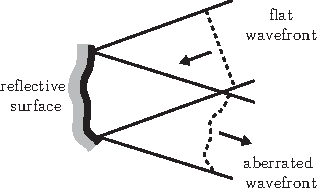
\includegraphics[width=\textwidth]{images/wavefront_distortions_reflection}
                \caption{Reflection.}
                \label{fig:abberation_reflection}
        \end{subfigure}
				\hspace{1em}
        \begin{subfigure}[b]{0.3\textwidth}
                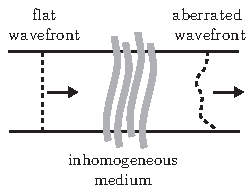
\includegraphics[width=\textwidth]{images/wavefront_distortions_transmission}
                \caption{Transmission.}
                \label{fig:abberation_trans}
        \end{subfigure}
        \caption{Wavefront aberrations due to (a) reflection from a non 
planar surface and (b)  caused by propagation through a non-uniform 
refractive index distribution~\cite{AOM_basic_ref}.}
\label{fig:abberations}
\end{figure} 

In biological microscopy, the two potential sources of aberrations are the optics and the specimen under study. Regarding the optics, one important parameter is the Numerical Aperture~(NA) since aberrations become more significant for those microscopes employing higher NA objectives. Aberrations can also be produced by the difference of refractive index between the microscope coverslip and the specimen mounting medium. Regarding the specimen, aberrations are caused by the variations in refractive index due to the three-dimensional nature of cells and tissue structures. These sample induced aberrations generally become dominant when the image focus lies deep within the sample, since light hast to pass a large distant trough an inhomogeneous medium~\cite{AOM_basic_ref}. 

There are different ways to characterize the aberrations mathematically. In systems with circular symmetry~(circular apertures) it is very common to use the Zernike polynomials because they form a complete, orthogonal set of functions defined over a unit circle~\cite{Zernike_original}:
\begin{align}
	\ W(\rho,\phi) = {\sum_{n}^{k}}{\sum_{m=-n}^{m=n}}{{c_n}^m {Z_n}^m}{(\rho,\phi)},
	\label{eq:aberration_zernike}
\end{align}
where $W(\rho,\phi)$ is the wavefront aberration function in polar coordinates at the exit pupil, $c_n^m$ are the Zernike coefficients and $Z_n^m (\rho,\phi)$ are the Zernike modes~(or polynomials). As we can see in the equation, the wavefront aberration function is a linear combination of polynomials. Therefore, the more polynomials~(i.e. modes, $Z_n^m (\rho,\phi)$) we can measure, the better characterization of the $W(\rho,\phi)$ function we have.
Representing aberrations in this way can simplify the design, control and characterization of the Adaptive Optics system. 

Although it is known where the aberrations come from, it is not always easy to measure them and implement the measure inside the optical system. There are different classifications of wavefront sensing in the bibliography~\cite{AO_engineering_handbook}. Here we will use the one employed by \emph{Martin J. Booth}~\cite{AOM_basic_ref} and we will explain the most common methods of wavefront sensing applied to microscopy.     
     
%%%%%%%%%%%%%%%%%%%%%%%%%%%%%%%%%%%%%%%%%%%%%%%%%%%%%%%%%%%%%%%%%%%%%%%%%%%%%%%
\subsection{Direct Wavefront Sensing}
\label{sec:WavefrontSensing}

Direct Wavefront Sensing is based on a direct measure of the phase gradient or the wavefront slope, it is considered as an aperture-plane sensing. Within this group there are several techniques such as interferometric, although in general the most used is the Shack-Hartmann. 

The Shack-Hartmann technique is based on a two-dimensional array of a few lenslets, a matrix of micro-lenses, all with the same diameter and the same focal length. The aberrated wavefront is divided into smaller sub-wavefronts and then imaged by the seperated micro-lenses onto a detector. The micro-lens matrix forms multiple focus spots in the focal plane and the recording device placed at the focal plane of the matrix records multiple spots, as shown in Fig.\ref{fig:SH}. The recording device is usually a CCD camera and typical micro-lens diameters range from about 100 to $\unit[600]{mm}$ with typical focal lengths ranging from a few millimeters to about $\unit[30]{mm}$~\cite{AO_vision_science}. By measuring the displacements~($\Delta x, \Delta y$) of each focal spot created by the separate microlenses~(Fig.~\ref{fig:SH}) allows to reconstruct the wavefront slopes and finally to reconstruct the wavefront aberration function.

\begin{figure}[htbp]
	\centering
		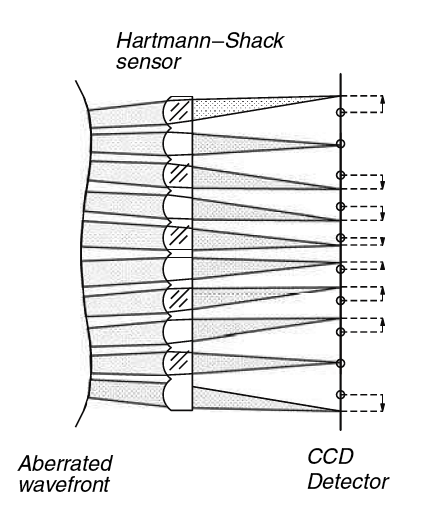
\includegraphics[width=0.30\textwidth]{images/SH}
	\caption{Two-dimensional section of Shack-Hartmann matrix of microlens. An incoming wavefront is divided in multiple, smaller sub-wavefronts and imaged onto a CCD~detector by a microlens array. This generates separate focal spots for each microlens. If the wavefront is not aberrated, each spot will be placed along the central axis of each microlens. If it is aberrated, it will be displaced with respect to this axis and a wavefront reconstruction can be performed based on the magnitude and direction if this displacement. Image after~\cite{optical_shop_testing}.}
	\label{fig:SH}
\end{figure}

While the basic idea of this sensing techniques is simple, we must note that a well defined wavefront in the pupil of the system is required which can only be produced by a point-like emitter. When studying three-dimensional, biological specimens, a single point like emitter is usually not encountered which leads to a number of problems. The first one is the superposition of wavefronts which depends on the coherence of the emitted light. Coherent light will cause interference in the pupil, thus causing ambiguous sensor readings rendering the measurement useless for aberration correction. 

If the specimen behaves as a point-like scatterer, it will emit incoherent light and the sensor is able to measure the aberrations produced in the emission path. If a reflection and not a transmission setup is used, the aberrations in the emission path shoud be the same as in the illumination path. However, if the specimen acts like a planar mirror in the focal region, the sensor will just be able to measure twice the even components of the aberrations produced in the illumination path~(or emission path). This is cause by the spatial inversion caused by any mirror, as shwon in Fig.~\ref{fig:abe_direct_sensing}). Hence we lose information part of the information about aberrations. Thus, implementing a direct sensing in this cases it is not a good option and indirect sensing schemes should be preferred.

\begin{figure}[htbp]
	\centering
		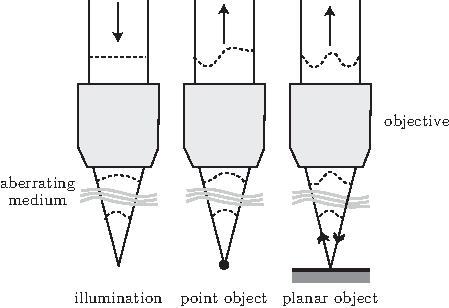
\includegraphics[width=0.50\textwidth]{images/abe_direct_sensing}
	\caption{Representation of the two effects due to the specimen structure on wavefront measurements. The left figure shows how the wavefront is aberrated in the illumination path. In the center it is shown a point-like scatterer. Only the emission path is measured. In the right figure it is shown a planar reflector. The illumination wavefront is spatially inverted on reflection before acquiring further aberration in the detection path. Image after~\cite{AOM_basic_ref}.}
	\label{fig:abe_direct_sensing}
\end{figure}

Another problem that can arise is due to three-dimensional nature of the specimen. The sensor might detect more signal intensity from the light scattered from out-of-focus areas rather than from the focal region. In order to overcome this problem, a spatial filter between objective and sensor can be used, much like the pinhole used in confocal microscopy. It is also possible to use coherence gating to exclude out-of-focus light instead of the spatial filter, although it is a more complex method~\cite{scan_TPFM_gated_wavefront}. 

%----------------------------------------------------------------------------
%%%%%%%%%%%%%%%%%%%%%%%%%%%%%%%%%%%%%%%%%%%%%%%%%%%%%%%%%%%%%%%%%%%%%%%%%%%%%
\subsection{Indirect Wavefront Sensing}
\label{sec:IndirectWavefrontSensing}

While direct wavefront sensing techniques are widely applied in astronomy, they are less common in microscopy techniques. This for several reasons. It is not as easy to create a ``guide-star`` like point source in a biological specimen. If there are no features in the specimen that occur naturally and which resemble a point source, one has to be implemented them manually which might alter the function of the specimen or might even be toxic to the sample. Modern microscopes are also highly complex and optimized, which makes it difficult to insert a relatively large wavefront sensor. For samples with weak signal strength, it is also desirable to collect as many photons as possible for the imaging process. Splitting the beam and using a part of the light emitted from the sample for direct wavefront sensing might hence decrease the signal strength or increase the recording time too much.

Indirect techniques do not measure the wavefront directly but instead optimize some merit function~(also called quality metric) that depends on the optical system. Indirect methods are used more often in industrial and medical applications. They usually require very little additional hardware. Once the technique is optimized for a specific problem, indirect schemes are easier to implement in practice and are more prone to errors due to the lack of additional hardware~(a single deformable mirror might be sufficient to implement adaptive optics in an existing microscope). 

For these techniques, the optimization of an image quality metric is mainly a mathematical rather than a technical problem. The aberration correction is performed through an iterative optimization of an image quality metric. The metric is usually based on spatial frequencies~\cite{wide_AOM_loew_freq} or image intensity~\cite{indirect_metric_intensity} and gives a mathematical measurement of how ``good'' the recorded image is. In many practical systems aberrations can be accurately represented by a small number of modes of an orthogonal basis, such as Zernike polynomials. The optimization is then performed by adapting the polynomial coefficients applied to the deformable mirror either stochastically or by using an appropriate mathematical model.

For the stochastic methods there are several algorithms, one of the most popular being genetic algorithms~\cite{Genetic_tutorial}. These algorithms try to find an optimal solution by simulating an evolution process. The implementation of a genetic algorithm in AO begins with a population of typically random sets of Zernike polynomials, called initial population. The separate members of the population are called chromosome~(also called genotype). After creating this initial population, each chromosome is evaluated and assigned a fitness value using the image quality metric. Then, a selection is applied to the population to create an intermediate population in a way that those chromosomes which represent a better solution are given more chances to ``reproduce'' than those chromosomes which are poorer solutions. Then recombination and mutation are applied to the intermediate population to create the next population. The process of going from the current population to the next population constitutes one generation. This process is repeated until a sufficiently good solution is found. These genetic algorithms do not require any preliminary information about the system but they are more time consuming than model-based approaches. Genetic algorithms are highly complex and a detailed description of the underlying principles and the separate steps is well beyond the scope of this report. We refer to \cite{Genetic_tutorial,Genetic_Algor1,Genetic_Algor2,Genetic_Algor3}for an in depth introduction as well as various applications of genetic algorithms in AO.

Methods based on a mathematical model acquire a sequence of images, each with a different, predefined aberration applied. The correction aberration is estimated from the information in this images and this process is repeated until the image quality is considered acceptable. The number of measurements needed to obtain an acceptable image depends strongly upon the optimization algorithm and parameters used, the mathematical representation of the aberration, and the object structure. For the earliest and most generic algorithms the number of measurements per aberration mode increases quadratically or exponentially with $N$, the number of corrected aberration modes~\cite{wide_sphere_packing}. The so called direct maximization method~(as described in Section~\ref{sec:TransmissionMicroscope}) is significantly more efficient, requiring only $2N+1$ measurements for $N$ mode. With this technique, Lukosz polynomials~\cite{wide_Lukosz_Modes} are used to classify the aberrations. The effects of different modes can then be separated and the optimization of each mode becomes independent and hence more efficient.

An effective model-based adaptive optics scheme should also be independent of the imaged object and should permit the separation of aberration and object influences on the measurements. This separation is also possible through the appropriate choice of optimization metric and aberration representation~\cite{wide_AOM_loew_freq}. The interested reader will find more information on the mathematical background in reference~\cite{wide_parabolic_optimization,wide_sphere_packing,wide_Lukosz_Modes,wide_AOM_loew_freq}. 


%%%%%%%%%%%%%%%%%%%%%%%%%%%%%%%%%%%%%%%%%%%%%%%%%%%%%%%%%%%%%%%%%%%%%%%%%%%%%%%
\subsection{Aberration Correction}
\label{sec:AberrationCorrection}

The wavefront correctors are an essential part of an adaptive optics system. The goal is to apply a certain phase profile to the incident wavefront by changing either the physical length over which the wavefront propagates or the refractive index of the medium through which the wavefront passes. Wavefront correctors are build using either mirrors or liquid crystals. The former apply the the phase change by adjusting their surface shape~(i.e., change their physical length while keeping the refractive index constant) while the latter keep the physical length constant and rely on localized changes in refractive index.  Mirror-based correctors are wavelength and polarization independent and can be reconfigured at rates of a few kilohertz~\cite{AOM_basic_ref}. They can have a continuous surface~(i.e., discrete actuator, bimorph or membrane mirrors) or segmented surface~(i.e. piston-only or piston/tilt mirrors) as shown in Fig.~\ref{fig:Correctors}. Unlike continuous mirrors, the segmented mirrors have gaps between the segments that reduce the efficiency and quality of the correction, although they can achieve much better wavefront fitting. 

\begin{figure}[tbh]
			\centering
			\begin{subfigure}[b]{0.25\textwidth}
							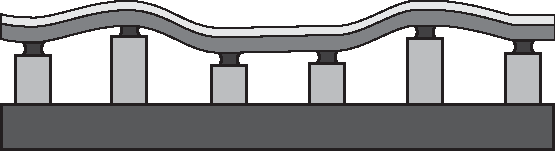
\includegraphics[width=\textwidth]{images/deformable_discrete}
							\caption{Discrete}
							\label{fig:Correctors_discrete}
			\end{subfigure}
			\quad
			\begin{subfigure}[b]{0.25\textwidth}
							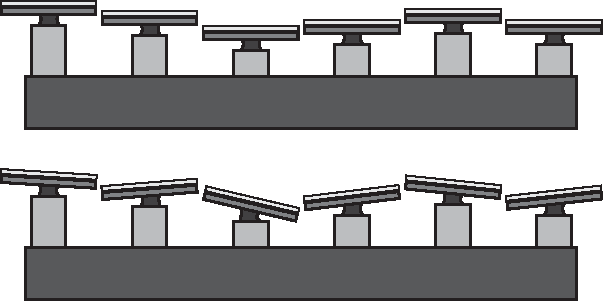
\includegraphics[width=\textwidth]{images/deformable_piston}
							\caption{Piston-Only}
							\label{fig:Correctors_piston}
			\end{subfigure}
			
			\vspace{5mm}
			
			\begin{subfigure}[b]{0.25\textwidth}
							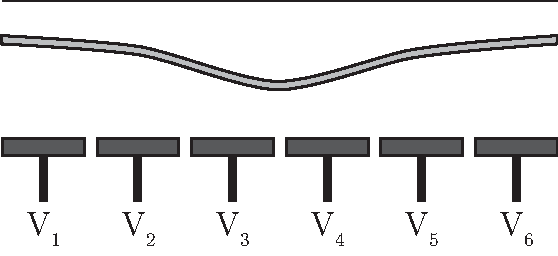
\includegraphics[width=\textwidth]{images/deformable_membrane}
							\caption{Membrane}
							\label{fig:Correctors_membrane}
			\end{subfigure}
			\quad
			\begin{subfigure}[b]{0.25\textwidth}
							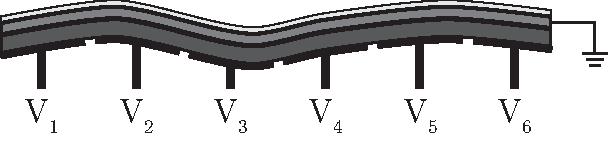
\includegraphics[width=\textwidth]{images/deformable_bimorph}
							\caption{Bimorph}
							\label{fig:Correctors_bimorph}
			\end{subfigure}							
			\caption{The four main mirror correctors. (a) Discrete actuator deformable mirrors consist of a continuous, reflective surface and an array of actuators, each capable of producing a local deformation in the surface. (b) Piston-only segmented correctors consist of an array of small planar mirrors whose axial motion~(piston) is independently controlled. Piston/tip/tilt-segmented correctors add independent tip and tilt motion to the piston-only correctors. (c) Membrane mirrors and (d) Bimorph mirrors. Image after~~\cite{AO_vision_science}.}
	\label{fig:Correctors}
\end{figure} 


Liquid crystal-based modulators change the refractive index electronically or optically, are wavelength and polarization dependent and can reach velocities of just a few tens of hertz. The nematic liquid crystal is the most common for AO applications. In general, they are much cheaper than the mirror-based correctors, are capable of producing more complex phase patterns but they have lower light efficiency due to absorption.   

In AO microscopes the first choice in most cases is the deformable mirror because of the higher efficiency. Furthermore, they are better suited for fluorescence techniques due to their polarization independent behavior. However, in particular cases, liquid-crystal modulators can be sufficient if aberration correction is only needed in the illumination path.
